\documentclass[twoside,11pt]{article}

%% Packages required by JSATsample
\usepackage{jsat}
\usepackage{amsmath,amsthm,amssymb}
\usepackage{pstricks}
\usepackage{pst-tree}

\input epsf
\special{papersize=8.5in,11in}

%% Other standard macros
\usepackage{amsfonts}
\usepackage{stmaryrd}
\usepackage[T1]{fontenc} %% needed to combine textsc with textbf

%% Figures
\usepackage{graphicx}
%\usepackage{tikz}
%\usetikzlibrary{positioning,shapes,shadows,arrows}
%\usetikzlibrary{decorations.pathmorphing,snakes}
%\usepackage{tkz-graph}
%\usepackage{wrapfig}

%% Hyperlinked references
\usepackage{hyperref}

%% Local macros
\newcommand{\sep}{.\,}
\newcommand{\limp}{\Rightarrow}
\newcommand{\posep}{*}
\newcommand{\points}{\mapsto}

\newcommand{\vars}{\mathit{Vars}}
\newcommand{\lvars}{\mathit{LVars}}
\newcommand{\rtypes}{\mathcal{R}}
\newcommand{\pfields}{\mathbb{F}}
\newcommand{\preds}{\mathbb{P}}
\newcommand{\loc}{\mathit{Loc}}
\newcommand{\model}[1]{\left[\!\left[#1\right]\!\right]}

\newcommand{\cdr}{\mathtt{tl}}
\newcommand{\lemp}{\mathit{lemp}}
\newcommand{\nil}{\mathtt{nil}}

\newcommand{\ls}{\mathtt{ls}}
\newcommand{\dll}{\mathtt{dll}}
\newcommand{\nll}{\mathtt{nll}}
\newcommand{\nlcdl}{\mathtt{nlcdl}}
\newcommand{\nlcl}{\mathtt{nlcl}}
\newcommand{\ndll}{\mathtt{ndll}}
\newcommand{\skl}{\mathtt{skl}}


\newcommand{\SLRD}{\textsc{SLID}}
\newcommand{\SLNL}{\textsc{SLNL}}
\newcommand{\SLL}{\textsc{SLL}}
\newcommand{\sllsat}{\texttt{sll}($\models$)}
\newcommand{\sllent}{\texttt{sll}($\limp$)}
\newcommand{\FDBent}{\texttt{FDB}($\limp$)}
\newcommand{\UDBsat}{\texttt{UDB}($\models$)}
\newcommand{\UDBent}{\texttt{UDB}($\limp$)}

\newcommand{\ASTERIX}{\textsc{Asterix}}
\newcommand{\CYCLIST}{\textsc{Cyclist-SL}}
\newcommand{\SLEEK}{\textsc{Sleek}}
\newcommand{\SLIDE}{\textsc{Slide}}
\newcommand{\SLSAT}{\textsc{SlSat}}
\newcommand{\SPEN}{\textsc{Spen}}

\newcommand{\smtlib}{\textsf{SMT-LIB}}
\newcommand{\smtcomp}{\textsf{SMT-COMP}}
\newcommand{\slcomp}{\textsf{SL-COMP}}
\newcommand{\starexec}{\textsf{StarExec}}

%%%%%%%%%%%%%%%%%%%%%%%%%%%%%%%%%%%%%%%%%%%%%%%%%%
% Header
%%%%%%%%%%%%%%%%%%%%%%%%%%%%%%%%%%%%%%%%%%%%%%%%%%
\jsatheading{1}{2014}{XX-YY}
\ShortHeadings{Report on SL-COMP 2014}
{M. Sighireanu and D.R. Cok}
\firstpageno{1}

%%%%%%%%%%%%%%%%%%%%%%%%%%%%%%%%%%%%%%%%%%%%%%%%%%
% Title
%%%%%%%%%%%%%%%%%%%%%%%%%%%%%%%%%%%%%%%%%%%%%%%%%%
\title{Report on \slcomp\ 2014}
\author{\name Mihaela Sighireanu \email sighirea@liafa.univ-paris-diderot.fr \\
        \addr LIAFA, University Paris Diderot \& CNRS \\
        \AND
        \name David R. Cok \email dcok@grammatech.com \\
        \addr GrammaTech, Inc., }
         %%
%by institution
%%Nikos Gorogiannis, Middlesex University London
%%Juan Navarro Perez, University College London
%%Adam Rogalewicz, Ondrej Lengal, Tomas Vojnar, FIT, Brno University of Technology, IT4Innovations Centre of Excellence, Czech Republic
%%Wei Ngan Chin, Le Quang Loc,  National University of Singapore
%%Radu Iosif, VERIMAG, CNRS, France
%%Andrey Rybalchenko, Microsoft Research
%%Constantin Enea, Mihaela Sighireanu, University Paris Diderot and CNRS
\date{\today}


\begin{document}

\sloppy
%%%%%%%%%%%%%%%%%%%%%%%%%%%%%%%%%%%%%%%%%%%%%%%%%%
% Title
%%%%%%%%%%%%%%%%%%%%%%%%%%%%%%%%%%%%%%%%%%%%%%%%%%
\maketitle

% Full articles by competition organizers reporting on SAT-related competitions within FLoC Olympic Games 2014. The articles should describe the competition, its criteria, why it is interesting to the SAT research community, execution environment used, analysis of the results (including how they compare to previous instantiations, if appropriate), and give a summary of the main technical contributions to the field, as well as discussions on lessons learned and suggestions for improvements for future competitions. 

%%%%%%%%%%%%%%%%%%%%%%%%%%%%%%%%%%%%%%%%%%%%%%%%%%
\begin{abstract}
A competition of solvers for Separation Logic 
was held in May 2014, 
as an unofficial satellite event of the FLoC Olympic Games.
%% like the OFF of a festival, i.e., un-official event
%% with the logistic support of \smtcomp. 
Six solvers participated in the competition; the success and performance
of each solver was measured over an appropriate subset of a library of benchmarks
accumulated for the purpose.
The benchmarks consisted of satisfiability and entailment problems
over formulas in the fragment of symbolic heaps with inductive definitions, 
which is the fragment of Separation Logic that is most used in program analysis and verification tools.
% These benchmarks are mainly crafted and come from the testing suits of the participating solvers.
%% DONE: Reviewer 2: remove comment on the use of SAT/SMT solvers by the SL solvers.
We report in this paper on 
the competition rules, the participants, the results, the findings, and  
the future of this event.
\end{abstract}


\keywords{Separation Logic, \smtlib, SAT Modulo Theory}

\published{December 12th, 2014}{\today}{}



%%%%%%%%%%%%%%%%%%%%%%%%%%%%%%%%%%%%%%%%%%%%%%%%%%
\section{Introduction}

Separation Logic (SL) is an established and fairly popular Hoare logic 
for imperative, heap-manipulating programs, 
introduced nearly fifteen years ago by Reynolds~\cite{Reynolds99,OHearnRY01,Reynolds02}. 
%
Its high expressivity, its ability to generate compact proofs, and 
its support for local reasoning 
have motivated the development of tools for automatic reasoning about programs using SL.
For a rather exhaustive list of the past and present tools, see the web site~\cite{OHearn-SLsite}.

These tools seek to establish memory safety properties and/or infer shape properties of the heap at a scale of millions of lines of code.
They intensively use (semi-)decision procedures for checking satisfiability and entailment problems in SL.
% in order to check Hoare's triples or to help the termination of a static analysis.
In the last five years, several papers reported on the design and implementation of such (semi-)decision procedures and compared publicly available tools~\cite{HasseIOP13}.

The organization of a public competition of SL solvers was an opportunity 
to collect the existing benchmarks and  
to make available the binaries of these solvers on a common platform, i.e., \starexec~\cite{StarExecsite}.
The \slcomp\ 2014 has been possible due to the support of the \smtcomp\ organizing committee, 
although SL is not a theory of the \smtlib\ format.
The competition has been held as an ``off'' (unofficial) event\footnote{That is, the competition was executed in conjunction with the games by the \smtcomp\ organizing committee, \smtcomp\ being an official participant in the games; the results of \slcomp\ 2014 were reported at the SMT-2014 workshop at FLoC; however, \slcomp\ 2014 was organized too late and was too experimental to be an official part of the FLoC Olympic Games.}
associated with the \smtcomp\ 2014 competition~\cite{SMTCOMPsite}, at the FLoC Olympic Games.
%% The results of the competition have been presented in the SMT workshop.
%%Informations about the participants and the final results are also available online at \url{www.liafa.univ-paris-diderot.fr/slcomp14/}.


%%%%%%%%%%%%%%%%%%%%%%%%%%%%%%%%%%%%%%%%%%%%%%%%%%
\section{Input Theory}
\label{sec:SL}

The competition focused on a fragment of SL that has been found to be the kernel of most tools, known 
as
the \emph{symbolic heaps} fragment
or Separation Logic with Inductive Definitions (\SLRD)~\cite{IosifRS13} or
the positive flat SL fragment~\cite{AntonopoulosGHKO14}. 
We provide here only an informal description of this fragment, its detailed description could be found in, e.g., \cite{Reynolds02,IosifRS13,AntonopoulosGHKO14}.  

%% DONE: Reviewers 1-3: provide informal description of the logic and references for the detailed description.
This fragment specifies the configurations of programs manipulating variables that are references to some record types; the records are defined by the user as a set of reference fields.
Such configurations are modeled by
(i) a heap that is a set of records and
(ii) a stack that maps program variables into \emph{locations} that are record addresses.
%
%% DONE: Reviewer 1: introduce alphabets
In the following, we denote by lower case letters $x,y,z$ the program variables and by upper case letters $X,Y,Z$ logical variables. The program variable $\nil$ has a fixed meaning representing an undefined (not allocated) location.
%
Variables and formulas are typed based on the user-defined records. Record values are denoted by mappings of record fields to locations stored in variables. For example, $\{(\texttt{lson},y), (\texttt{rson},z)\}$ denotes a value for a record defining a binary tree node.

The (non-)aliasing relation between variables are specified using (dis-)equality atoms, e.g., $x = y$ or $x\neq z$. A conjunction of such atoms is called a \emph{pure formula}. 
%
The heap is specified using three kinds of atomic propositions, called also \emph{spatial atoms}:
(i) the empty heap $\mathit{emp}$, 
(ii) a heap consisting of one allocated record which location is stored in some variable, e.g., $x \points \{(\texttt{lson},y), (\texttt{rson},z)\}$,
and
(iii) an unbounded heap segment allocated for a data structure whose shape is defined by an \emph{inductive definition}.
Table~\ref{tab:RD} provides some examples of such inductive definitions. 
The spatial atoms are connected via the \emph{separating conjunction operator} $\posep$ to form a \emph{spatial formula}. 
A formula in \SLRD\ is the conjunction of a pure and a spatial formula.

For example, the following formula specifies a heap built from two cells of a singly linked list
(with locations stored in $x$ resp. $y$) and a list segment (starting from $z$ and ending in $y$):
\begin{align}
x \points \{(\texttt{nxt},y)\} \ \posep\ y \points \{(\texttt{nxt},\nil)\} \ \posep\ \ls(z,y)
\end{align}
The definition of $\ls$ in Table~\ref{tab:RD} specifies acyclic and possibly empty singly linked list segments starting in $E$ and with last element pointing to $F$.
The list is acyclic due to the non-aliasing pure constraint $E\neq F$ which prevents $F$ to be one of the cells inside the list segment.
%
%% DONE: Reviewer 1: better integration of examples in the text 
%% DONE: Reviewer 2: fill the space around Table 1
%% DONE: Reviewer 3: explain at least one of the ID in Table 1
We explain in the following the inductive definitions in Table~\ref{tab:RD}.
%
The atom $\nll(E,F,B)$ specifies a list segment (of successor field \texttt{nxtup}) starting from $E$ where each cell has a reference (in field \texttt{inner}) to a list segment ending in some common border location $B$. 
%
The definition $\dll(E,L,P,F)$ specifies a doubly linked list segment rooted at $E$ and ending in $L$; $P$ denotes the previous location of $E$ (stored in field \texttt{prv}) and $F$ denotes the next location of $L$  (stored in field \texttt{nxt}).
%
The definition $\mathtt{btree}(E)$ specifies a binary tree with root $E$:
the first disjunct defines the case of an empty tree, i.e., with $\nil$ root, while the second disjunct defines a tree with at least one cell allocated at $E$ separated from the trees rooted in its locations stored in the fields \texttt{lson} and \texttt{rson}.
%
This simple definition of binary trees is extended in $\mathtt{tll}$ to keep track of the parent node in each cell and to link the leaves of the tree into a singly linked list (between $E$ and $F$) using the \texttt{nxt} field.
%
The general syntax of the inductive definitions is the following:
\begin{equation}\label{eq:RD}
P(\vec{E}) \triangleq \bigvee_i \exists \vec{X}_i\sep \Pi_i \land \Sigma_i
\end{equation}
\noindent where $\Pi_i$ (resp. $\Sigma_i$) is a pure (resp. spatial) formula over parameters $\vec{E}$ and variables in $\vec{X}_i$.
Notice that the existential quantification and disjunction are allowed only in inductive definitions. 
Also, the semantics chosen in the competition is the \emph{precise} semantics.


\begin{table}
\begin{eqnarray}
%
\lefteqn{\textit{singly linked lists}} \nonumber \\
\ls(E,F) & \triangleq & (E=F\land\mathit{emp}) \lor (E\neq F \land 
\exists X\sep E\points\{(\texttt{nxt},X)\}\ \posep\ \ls(X,F)) 
\\[1mm]
%  
\lefteqn{\textit{nested linked lists}} \nonumber \\ 
\nll(E,F,B) & \triangleq & (E=F\land\mathit{emp}) \lor (E\neq F \land E\neq B \land \\
&& \exists X,Z\sep E\points\{(\texttt{nxtup},X),(\texttt{inner},Z)\}\ \posep\ \ls(Z,B)\ \posep\ \nll(X,F,B)) \nonumber
\\[1mm]
%  
\lefteqn{\textit{doubly linked lists}} \nonumber \\ 
\dll(E, L, P, F) & \triangleq & (E=F\land L=P\land \mathit{emp}) \lor \big( E\neq F \land L\neq P \land \\
&& \exists X\sep E\points \{(\texttt{nxt},X),(\texttt{prv},P)\}\ \posep\ \dll(X,L,E,F)\ \big)\nonumber
\\[1mm]
%  
\lefteqn{\textit{binary tree}} \nonumber \\ 
\mathtt{btree}(E) & \triangleq & (E=\nil\land \mathit{emp}) \lor \big( E\neq \nil \land 
\\
&& \exists X,Y\sep E\points \{(\texttt{lson},X),(\texttt{rson},Y)\}\ \posep\ \mathtt{btree}(X)\ \posep\ \mathtt{btree}(Y)\big)
\nonumber 
\\[1mm]
%  
\lefteqn{\textit{tree with linked leaves}} \nonumber \\ 
\mathtt{tll}(R,P,E,F) & \triangleq & (R=E \land R\points \{(\texttt{lson},\nil),(\texttt{rson},\nil),(\texttt{parent},P),(\texttt{nxt},F)\}) ~\lor~ \\
&&\big( R\neq E \land \exists X,Y,Z\sep 
\begin{array}[t]{l}
R\points \{(\texttt{lson},X),(\texttt{rson},Y),(\texttt{parent},P),(\texttt{nxt},Z)\} \posep \\
\mathtt{tll}(X,R,E,Z)\ \posep\ \mathtt{tll}(Y,R,Z,F)\big)
\end{array} \nonumber  
\end{eqnarray}
\caption{Examples of inductive definitions used in the benchmark}
\label{tab:RD}
\vspace{-3eX}
\end{table}

%%%%%%%%%%%
%\paragraph{Syntax:}
%Let $\pfields$ be a finite set of \emph{field names} used in the definition of records.
%The set of \emph{program variables} is denoted by $\vars$ and we use lower-case letters $x, y, z$ for them.
%The \emph{logical variables} are denoted by capital letters in an alphabet $\lvars$.
%Inductive definitions use names in a finite set $\preds$.
%The syntax of formulas in the symbolic heaps fragment of Separation Logic
%is given by the following grammar:
%$$
%\begin{array}{c}
%\begin{array}{ll}
%f \in \pfields \mbox{ field names} ~&~
%P \in \preds \mbox{ inductive definition name}
%\\[0.8mm]
%x,y \in \vars \mbox{ program variables} ~&~
%X,Y \in \lvars \mbox{ logical variables}
%\end{array}
%\\[2mm]
%%
%%
%E,F\ ::=\ x \mid X 
%\hfill \mbox{variables}
%\\[1mm]
%\rho\ ::=\ \{ (f,E) \} \mid \rho\cup\rho 
%\hfill \mbox{set of field references}
%\\[2mm]
%%
%% pure part
%\Pi\ ::=\ E = F \mid E \neq F \mid \Pi \land \Pi \hfill 
%\mbox{pure formulas}\\[1mm]
%%
%% spatial part
%\Sigma\ ::=\
%\mathit{emp} \mid
%E \points \rho \mid 
%P(\vec{E}) \mid 
%\Sigma \posep \Sigma 
%%
%\hspace{1cm}\hfill \mbox{spatial formulas}
%\\[2mm]
%A,B\ \triangleq\ \exists \vec{X}\sep \Pi\land\Sigma \hfill \mbox{formulas} %
%\end{array}
%$$

%%%%%%%%%%%
%\paragraph{Semantics:}
%Let $\loc$ be a set of locations. 
%A stack $S : \vars\cup\lvars\rightarrow \loc$ maps
%variables to locations. 
%A heap $H:\loc\times\pfields\rightharpoonup\loc$ is a partial
%function that defines values of fields for some of the locations in $\loc$.
%%
%The domain of $H$ is denoted by $\mathit{dom}(H)$ and
%the set of locations in the domain of $H$ is denoted by $\mathit{ldom}(H)$.  
%As expected, $\nil$ is interpreted to a location $S(\nil)\not\in \mathit{ldom}(H)$.
%
%The set of configurations satisfying a formula $\varphi$ is defined by the relation
%$(S,H)\models \varphi$ defined in Table~\ref{tab:sem} ($\uplus$
%denotes the disjoint union of sets and $S[X\gets\ell]$ denotes the function
%$S'$ s.t.  $S'(X)=\ell$ and $S'(Y)=S(Y)$ for any $Y\neq X$).
%Note that a configuration $(S,H)$ satisfies a predicate atom 
%$P(\vec{E})$ if it belongs to the least fixed point of the set of inductive definitions $\preds$ for the actual parameters $\vec{E}$ of $P$.
%The set of models of a formula $\varphi$ is denoted by $\model{\varphi}$. Given two
%formulas $\varphi_1$ and $\varphi_2$, we say that $\varphi_1$ entails
%$\varphi_2$, denoted by $\varphi_1\limp\varphi_2$, iff
%$\model{\varphi_1}\subseteq \model{\varphi_2}$. 
%%
%Notice that this semantics is a \emph{precise} semantics. It was chosen because it is the most used in tools and in the verification of concurrent programs.
%%%give more details on difference between intuitionistic/precise, 
%%%why precise? needed for concurrent program analysis
%
%
%
%\begin{table}
%\begin{center}
%%\begin{footnotesize}
%\begin{tabular}{lcl}
%$(S,H) \models E=F$ & iff &  $S(E)=S(F)$
%%, where $\model{x}_{S,I}= S(x)$ and $\model{X}_{S,I}= I(X)$ for $x \in \vars$,
%% $X \in \lvars$
%\\[.5mm]
%$(S,H) \models E\ne F$ & iff &  $S(E)\neq S(F)$ \\[.5mm]$(S,H) \models \varphi\land\psi$ & iff &  $(S,H) \models \varphi$ and $(S,H) \models \psi$ \\[.5mm]
%$(S,H) \models \mathit{emp}$ & iff & $\mathit{dom}(H)=\emptyset$
%\\[.5mm]
%$(S,H) \models E\points \{\rho\}$ & iff &
%  $\mathit{dom}(H)=\{(S(E),f_i)\mid (f_i,E_i)\in \{ \rho \} \}$ and\\[.5mm]
%  & & for every $(f_i,E_i)\in \{ \rho \}$, $H(S(E),f_i)=S(E_i)$
%\\[.5mm]
%%%MS: per-object separation of formulas
%$(S,H) \models \Sigma_1\posep\Sigma_2$ & iff & $\exists H_1,H_2$ s.t.
%  $\mathit{ldom}(H)=\mathit{ldom}(H_1)\uplus\mathit{ldom}(H_2)$,\\[.5mm]
%  & & $(S,H_1)\models\Sigma_1$, and $(S,H_2)\models\Sigma_2$
%\\[.5mm]
%%preds
%$(S,H) \models P(\vec{E})$ & iff &
%$(S,H)\in \model{\preds}(P(\vec{E}))$
%\\[.5mm]
%$(S,H) \models \exists X\sep\varphi$ & iff & there exists $\ell\in\loc$ s.t. $(S[X\gets\ell],H)\models \varphi$
%\end{tabular}
%%\end{footnotesize}
%\end{center}
%\caption{Semantics of the Separation Logic fragment}
%\label{tab:sem}
%
%\end{table}



%%%%%%%%%%
\paragraph{Decidability and complexity properties:}
The main difficulty that faces automatic reasoning using the symbolic heaps fragment is that the logic, 
due to its expressiveness, does not have very nice decidability properties~\cite{AntonopoulosGHKO14}.
For this reason, most program verification tools use incomplete heuristics to solve the satisfiability and entailment problems.
%
We summarize below the results obtained on the decidability of this fragment.
The various benchmarks and competition divisions introduced in \slcomp\ stem from these results.
\begin{description}
\item[\SLRD+:]
This fragment considers inductive definitions of the general form given in equation (\ref{eq:RD}).
Its satisfiability problem is decidable~\cite{BrotherstonFGNP13},
but the validity of an entailment is not~\cite{AntonopoulosGHKO14}.
%
%% Does they have disjunctions?
A sub-fragment of \SLRD+ that has a decidable entailment problem has been identified in~\cite{IosifRS13}. 
It includes \emph{bounded tree width} inductive definitions.
These definitions are general enough to define (doubly-) linked lists, trees,
and structures more general than trees, such as trees whose leaves are chained in
a list (i.e., $\mathtt{tll}$ in Table~\ref{tab:RD}). 
The restrictions in~\cite{IosifRS13} on the syntax allowed in equation (\ref{eq:RD}) are very technical. They require in substance that all models of such formulas have bounded tree width. 
In particular, they require that there is exactly one points-to predicate in any $\Sigma_i$ in equation (\ref{eq:RD}).
%% a stratification of the call graph of inductive definitions,
The entailment problem in this fragment is EXPTIME-hard~\cite{AntonopoulosGHKO14}.

\item[\SLNL:]
This fragment, formally defined in~\cite{EneaLSV14}, is obtained from \SLRD+ by mainly restricting the inductive definitions to nested lists data structures, and including skip-lists. 
This restriction allows to improve the complexity of the entailment problem to NPTIME. 

\item[\SLL+:]
This fragment is obtained when only the $\ls$ definition is used.
The entailment problem is $\Pi^P_2$-complete~\cite{AntonopoulosGHKO14}.

\item[\SLL:]
This is a sub-fragment of \SLL+ obtained by requiring that:
(i) both formulas of the entailment problem do not contain disjunctions and 
(ii) the right-hand side formula has no existential quantification\footnote{This is the case for the verification conditions generated for checking safety properties of programs.}. 
This sub-fragment has a PTIME decision procedure for the entailment problem~\cite{CookHOPW11}.
\end{description}

%% DONE: Reviewer 3: rephrase the comment on the divisions issued from the problems and results
\noindent
%Out of the 6 possible divisions (three classes of problems above and the two decision problems considered), 
%only five were opened because only one solver was available for checking satisfiability in the \SLL+ fragment.
The competition targeted the fragments \SLRD+, \SLNL, and \SLL. 
Out of the 6 possible divisions (the three fragments above and the two decision problems considered), only five were opened because only one solver was specialized for checking satisfiability in \SLNL.


%%%%%%%%%%%%%%%%%%%%%%%%%%%%%%%%%%%%%%%%%%%%%%%%%%
\section{Competition Organization}

The first edition of \slcomp\ focused on %two goals:
bringing together a large set of SL solvers and
building a common but not trivial benchmark suite. 

%%%%%%%%%%
\subsection{Launching procedure and support}
A call for participation and benchmarks was sent
in May 2014 %, May 14th 2014
to several research groups 
%%
that are actively developing solvers for SL.
The researchers that positively replied and some other researchers known for their work on tools for SL were invited to discuss the organization details on a public mailing list \url{smtcomp14-sl@googlegroups.com}.
%% DONE: Reviewer 1: odd sentence, please rephrase.
%We solicited the support of the chair of the \smtcomp\ 2014 organizing committee, David Cok, to benefit from his experience in the organization of such competitions.
The support of the officers of the \smtcomp\ 2014 organizing committee was solicited to benefit from their experience in the organization of such competitions.
%
A message describing the competition was sent on the \smtcomp\ and \smtlib\ discussion lists. Following this message, some members of the \smtcomp\ steering committee were added to the \slcomp\ discussion list. 
This inaugural edition of the competition was jointly organized by Mihaela Sighireanu and David Cok:
Mihaela Sighireanu enlisted participation, moderated the discussion on competition rules, and organized the 
collection, translation, and categorization of benchmarks; 
David Cok advised on the competition organization and rules based on experience with other competitions, and he executed and reported the results of the competition using the \starexec\ framework.


%%%%%%%%%%
\subsection{Participants}
Seven teams representing seven different solvers replied to the call for participation.
These teams provided:
(1) benchmarks, 
(2) a description of the input format of their solver, 
(3) a reference to a technical paper describing the principles used by the solver, 
%usually, it is not DPLL
(4) a web site, and
(5) a statically linked Linux binary which could be executed on the \starexec\ platform.
%
Because the time given for preparing the binary was very short (2 weeks), one solver~\cite{HasseIOP13}
%give details
retired from the competition. The problem faced by this solver will be discussed further in the concluding remarks.
%
Note that although one person is listed as ``submitter'' for a solver on the web site,
%give here generic web site or \url{www.smt-comp.org}, 
there is generally a team of contributors behind each tool; the identified person is simply the communication contact.
%
The participants in this first edition are described below.

%% TODO: Reviewer 2: the tool internal techniques is a bit short and could be extended
%\begin{itemize}
%\item \ASTERIX~\cite{PerezR13} solver 
\smallskip
\noindent
\textbf{\ASTERIX}~\cite{PerezR13}: 
was submitted by 
Juan Navarro Perez (UCL, UK) and 
Andrey Rybalchenko (Microsoft Research Cambridge, UK).
The solver deals with the satisfiability and entailment checking in the \SLL\ fragment.
For this, it implements a model-based approach.
The procedure relies on SMT solving technology (Z3 solver is used) to untangle potential aliasing between program variables. 
It has at its core a matching function that checks whether a concrete valuation is a model of the input formula and, if so, generalizes it to a larger class of models where the formula is also valid.  


%\item \CYCLIST~\cite{BrotherstonGP12,CYCLISTsite} solver 
\medskip
\noindent
\textbf{\CYCLIST}~\cite{BrotherstonGP12,CYCLISTsite}:
was submitted by 
Nikos Gorogiannis (Middlesex University London, UK).
%J. Brotherston, N. Gorogiannis, and R. L. Petersen 
The solver deals with the entailment checking for the \SLRD+ fragment.
It is an instantiation of the theorem prover \textsc{Cyclist} for the case of Separation Logic with inductive definitions. 
The solver builds derivation trees and uses induction to cut infinite paths in these trees
% with ``back-links'' from leaves to nodes of the tree 
that satisfy some soundness condition. 
For the Separation Logic, \CYCLIST\ replaces the rule of weakening used in first-order theorem provers with the frame rule of SL.


%\item \SLEEK~\cite{ChinDNQ12,SLEEKsite} solver 
\medskip
\noindent
\textbf{\SLEEK}~\cite{ChinDNQ12,SLEEKsite}:
was submitted by 
Quang Loc Le and Wei Ngan Chin (NUS, Singapore).
The solver deals with the satisfiability and entailment checking for \SLRD+ formulas.
It is an (incomplete but) automatic prover, that builds a proof tree for the input problem by using the classical inference rules and the frame rule of SL. It also uses a database of lemmas for the inductive definitions in order to discharge the proof obligations on the spatial formulas.
%
The proof obligations on pure formulas are discharged by external provers like CVC4, Mona, or Z3.

%\item \SLIDE~\cite{IosifRV14,SLIDEsite}  solver 
\medskip
\noindent
\textbf{\SLIDE}~\cite{IosifRV14,SLIDEsite}: 
was submitted by 
Adam Rogalewicz and Tomas Vojnar (VeriFIT, Czech Rep) and
Radu Iosif (Verimag, France).
The solver deals with the entailment problem in the decidable sub-fragment of \SLRD+ defined in~\cite{IosifRS13}.
The proof method for checking $\varphi\limp\psi$ relies on converting $\varphi$ and $\psi$ into two tree automata $A_\varphi$ resp. $A_\psi$, and checking
the tree language inclusion of the automaton $A_\varphi$ in the automaton $A_\psi$.

%\item \SLSAT~\cite{BrotherstonFPG14} solver 
\medskip
\noindent
\textbf{\SLSAT}~\cite{BrotherstonFPG14}:
was submitted by 
Nikos Gorogiannis (Middlesex University London, UK) 
and  Juan Navarro Perez (UCL, UK).
%J. Brotherston, C. Fuhs, N. Gorogiannis, and J. Navarro Perez
The solver deals with the satisfiability problem for the \SLRD+ fragment with general inductively defined predicates.
The decision procedure is based on a fixed point computation of a constraint, called the ``base'' of an inductive predicate definition. This constraint is a conjunction of equalities and dis-equalities between a set of free variables built also by the fixed point computation from the set of inductive definitions.

%\item \SPEN~\cite{EneaLSV14,SPENsite} solver 
\medskip
\noindent
\textbf{\SPEN}~\cite{EneaLSV14,SPENsite}:
was submitted by 
Mihaela Sighireanu (UPD \& CNRS, France).
%C. Enea, O. Lengal, M. Sighireanu, and T. Vojnar
The solver deals with satisfiability and entailment problems for the fragment \SLNL.
%\SLRD+ where 
%(i) the inductive definitions correspond to some class of (nested) lists
%and (ii) the right-hand side of the entailment problem does not have existential quantifiers.
%The class of inductive definitions allowed is included in the decidable fragment defined by~\cite{IosifRS13}, but is restricted to list segments in order to obtain an efficient decision procedure.
The decision procedures calls the MiniSAT solver on a boolean abstraction of the SL formulas to check their satisfiability and to ``normalize'' the formulas by inferring its implicit (dis)equalities. % implicit from the semantics of SL.
The core of the algorithm checking if $\varphi\limp\psi$ is valid searches a mapping from the atoms of $\psi$ to sub-formulas of $\varphi$.
This search uses the membership test in tree automata to recognize in sub-formulas of $\varphi$ some unfolding of the inductive definitions used in $\psi$.

%\end{itemize}

\medskip
A notable fact about this set of participants is the diversity of techniques used by each solver:
reduction to SAT or SMT problems (\ASTERIX, \SLSAT, \SPEN),
resolution based (\CYCLIST, \SLEEK),
reduction to finding graph homomorphism (\SPEN), and
reduction to tree automata membership test (\SPEN) or to tree automata inclusion test (\SLIDE).
%
Some of the above solvers deal with other problems than the ones considered for this competition, e.g., the computation of an unsatisfiability core or abduction.


%%%%%%%%%%
\subsection{Benchmarks and their input format}

%% DONE: Reviewer 3: comment the lack of industrial benchmarks
The set of benchmarks was built based on contributions from each participant. 
Some of these problems come from academic software analysis or verification tools based on SL 
(e.g., \textsc{SmallFoot}~\cite{SmallFootsite}, \textsf{Hip}~\cite{ChinDNQ12}).
But no problem issued from industrial tools was included in the benchmarks because we didn't receive such input.
The benchmarks were collected in the input format submitted by the participants. 
This set of problems was translated into a common format designed like a logic of the \smtlib\ format~\cite{BarST-SMTLIB}.
That is, they used the syntax of \smtlib v2, although the SL theory underlying the syntax is not an official \smtlib\ theory or, at this point, even compatible with the logic underlying \smtlib.
The rationale for this choice of common input format is 
that SL is combined with or translated into first-order theories that are or will be supported by the \smtlib\ format.
Also, we needed a typed input format and some support for processing this format\footnote{In particular, we used the parser for the \smtlib v2 available at \url{www.smtlib.org/utilities.html}.}.
 
\paragraph{Input format:} Each benchmark file is organized as follows:
\begin{itemize}
\item Preamble information required by the \smtlib\ format: the theory, the source, the kind (crafted, application, etc) and status of the problem.  Here the logic was designated as \textbf{QF\_S}, even though that is not at this point an official \smtlib\ logic. 
\item The set of sorts (records), fields, and inductive definitions used in the problem. Notice that the input format is strongly typed, i.e., each program variable has a unique type (reference to some sort) and 
fields are typed as function symbols from their declaration type to their definition type. 
\item One resp. two assertions for each satisfiability resp. entailment problem. 
\item The file ends with a checking satisfiability command\footnote{Checking the validity of the entailment $A\limp B$ is encoded by checking the satisfiability of its negation $A \land \lnot B$.}.
\end{itemize}

The syntax and semantics of this format were discussed and agreed in the public mailing group. 
The exact definition of the theory used and the full set of benchmarks is available on-line as a GITHUB archive\footnote{\url{github.com/mihasighi/smtcomp14-sl}}.

\paragraph{Selection process:} The final version of benchmarks was the result of several iterations of the following actions on the initial set of problems:
\begin{itemize}
\item We ensured that the semantics used in the input format of solvers matched the one used in the common format. 
For example, some solvers rejected problems with non-aliasing constraints ($x\neq y$) between variables of different sorts. The final input format required to deal with such constraints and to interpret them as valid.

\item The status (expected result), the source, and the kind of each problem were supplied as \smtlib\ meta-information.
\slcomp\ benchmarks are only crafted (i.e., demonstrates a particular aspect of a solver or problem domain) or
random (instance of a problem template parameterized on some dimension, e.g., a size).
%% DONE: removed the other kinds because not used.

\item The benchmark curation process identified some problems that had an incorrect expected result computed by their source solver, which required fixing the problem in the solver and in the benchmark.
%% DONE: Reviewer 2: Were any discrepancies found? What was the procedure to handle those?
The status of each problem was checked before the competition using at least two solvers and it did not change during the competition. 
\end{itemize}

\paragraph{Divisions:} The final benchmarks have the characteristics presented in Table~\ref{tab:bench}.
The benchmark set was split into five divisions, using the kind of problems solved and the kind of inductive definitions used (described in Section~\ref{sec:SL}), as follows:
\begin{description}
\item[\sllsat:] includes satisfiability problems for the \SLL\ fragment.
%%As mentioned before, this fragment has been identified to have a polynomial complexity for the satisfiability problem.
Most of problems in this division were provided by the team of the \ASTERIX\ solver in~\cite{PerezR11}.

\item[\sllent:] includes entailment problems for the \SLL\ fragment and has the same source. The problems were either randomly generated to prove the capabilities of the solver or they are verification conditions generated by the \textsc{SmallFoot} tool~\cite{SmallFootsite}.

\item[\UDBsat:] includes satisfiability problems for the \SLRD+ fragment, i.e., formulas using any fixed, user-defined set of inductive definitions satisfying the syntax given in equation (\ref{eq:RD}).
Recall that this problem is decidable. 
The problems were proposed by the teams of \SLSAT\ and \SLEEK\ solvers.

\item[\UDBent:] includes entailment problems for formulas in the \SLRD+ fragment.
Recall that this problem is undecidable. 
The problems were proposed by the teams of \CYCLIST, \SLEEK, \SLIDE, and \SPEN.

\item[\FDBent:] includes entailment problems for formulas in the \SLNL\ fragment. 
%using a fixed set of inductive definitions, mainly defining several kinds of nested, singly or doubly linked lists. 
Recall that this fragment is decidable. % in~\cite{AntonopoulosGHKO14,EneaLSV14}.
%Moreover, some solvers have very efficient procedures for such definitions.
The problems were proposed by the team of \SPEN.
\end{description} 
 
\begin{table}
\begin{center}
\begin{tabular}{p{6cm}r}\hline
\multicolumn{2}{c}{Total number of problems: 678} \\
\hline
Satisfiability & 25\% \\
Entailment & 75\% \\
\hline
%
\hline
\multicolumn{2}{c}{Origin} \\
\hline
Crafted & 41\% \\
Randomly generated & 59\% \\
\hline
%
\hline
\multicolumn{2}{c}{Problems by division} \\
\hline
\sllsat & 110 \\ %& 59\% \\
\sllent & 292 \\ %
\FDBent &  43 \\ %& 6\% \\ 
\UDBsat &  61 \\ %& 35\% \\
\UDBent & 172 \\
\hline
\end{tabular}
\end{center}
\caption{Final benchmark set}
\label{tab:bench}
\vspace{-3eX}
\end{table}


%%%%%%%%%%
\subsection{Competition infrastructure}

%% DONE: Reviewer 2 suggestion to group small paragraphs.
%%     the main idea being "details on competition parameters".
\slcomp\ used the \starexec\ platform~\cite{StarExecsite} under the control of David Cok 
%% more on the benefits of this platform
and required several features provided by this platform.
%
The pre-processing was used for 5 of the 6 solvers in order to translate the problems from the common format to the internal format of each solver. The code of these pre-processors is available on the competition GitHub repository.
%
The competition did not use the scrambling of benchmarks because the names used for inductive definitions defined in the files of some divisions (mainly, \sllsat, \sllent, and \FDBent\ divisions) are important for the solvers.
%
Each benchmark file included only one problem. 
The incremental feature was not used and is not supported by most of the competing solvers.
%
\starexec\ imposes a time and space limit on each attempt of a solver to solve a given benchmark. For this competition, the CPU time\footnote{None of the participating solvers was parallel.} was limited to 2400 seconds and
the memory (RAM) limit was 100GB. 
%% DONE: Reviewer 3: comment the limits and specify if parallel solvers involved.
Some jobs did have CPU timeout or reached the memory limit.
%% TODO: see why David changed this?
%%       However, no benchmark problem was complex enough to even approach these limits.
%
%% DONE: Reviewer 2: comment on training runs and how discrepancies have been fixed
The participants trained their solvers on the platform and provided feedback where the expected result of a problem did not match their result. Several benchmarks and solvers were fixed during this period.
One training run was executed before the official run to provide insights about the global results and to do a final check of the benchmarks.

The computation of the scores obtained for each division followed the rules fixed for \smtcomp'14.
The best score is the one with, in order:
(a) the least number of incorrect answers, 
(b) the largest number of correctly solved problems, and 
(c) the smallest time taken in solving the correctly solved problems.
%
Note that solvers are allowed to respond ``unknown" or to time-out on a given benchmark without penalty (other than not being able to count that benchmark as a success).
Note also that a single wrong answer, even accompanied by many correct answers, places a competitor behind one that has just one right answer. This choice is intended to emphasize the need for sound, bug-free solvers that can be relied upon by an application-focused user community. 
%
Giving the number of correctly
solved problems priority over the time taken to solve them is a more debatable choice. To date the emphasis in these competitions has been on raw logical capability of a solver; however, many applications are more concerned with fast solutions of most problems rather than eventual solution of more problems. Thus the scoring metric may be reconsidered for future competitions.




%%%%%%%%%%%%%%%%%%%%%%%%%%%%%%%%%%%%%%%%%%%%%%%%%%
\section{Results}

\begin{table}
\begin{center}
%\begin{tabular}{p{2.5cm}p{2cm}p{2cm}p{2cm}p{2cm}p{2.5cm}}\hline
\begin{tabular}{l*{5}c}\hline
\multicolumn{1}{r}{\emph{Division}} & \sllsat & \sllent & \FDBent & \UDBsat & \UDBent \\
\multicolumn{1}{r}{\emph{size}} & 110 & 292 & 43 & 61 & 172 \\
\hline
\ASTERIX &
\textbf{110/1.06} &  %1
\textbf{292/2.98} &  %1
-- &
-- &
--
\\\hline
\CYCLIST &
-- &
55/11.78 & %4
19/141.78 & %2
-- &
\textbf{120/145.33} %1
\\\hline
\SLEEK &
110/4.99 & %3
292/14.13 & %3
31/43.65 [\emph{1}] & %3
\textbf{61/30.84} & %1
131/80.60 [\emph{4}] %3
\\\hline
\SLIDE &
-- &
-- &
-- &
-- &
36/195.61 %2
\\\hline
\SLSAT &
55/0.55 [\emph{55}] & %4
--  &
--  &
37/2620.52 & %2
--
\\\hline
\SPEN &
110/3.27 & %2
292/7.58 & %2
\textbf{43/0.61} & %1
-- &
--
\\\hline
\end{tabular}
\end{center}
\caption{%
%% DONE: Reviewer 2: add the incorrect answers
%% DONE: Reviewer 3: specify times
Overall results $n/t~[f]$ where %
$n$ is the number of solved problems,  %
$t$ is the cumulated CPU time (sec) on solved instances, %
$f$ is the number of incorrect answers, if any %
%(1=first place, 2 = second place, etc.)
}
\label{tab:overall}
\vspace{-3eX}
\end{table}


\paragraph{New benchmarks:}
One of the goals of \slcomp\ was to build an interesting set of benchmark problems. 
Aside from its use in the competition, the current set provides a reference of the kind of problems handled efficiently by the existing solvers and techniques.
Moreover, researchers can use the collected benchmarks for the evaluation of competing solvers and for the testing of their own solver quite apart from any competition. 
In particular, it was important to obtain benchmarks relevant to the actual application area, i.e., software verification.

\paragraph{Publicly available solvers:} \starexec\ requires that a public version of a solver be made available on \starexec\ as a condition of participating in a competition. This allows users of \starexec\ to rerun a competition if so desired. More importantly, it allows users to upload a new set of benchmarks of interest in their application domain and to try the various solvers against those benchmarks.

\paragraph{Overall results:}
Table~\ref{tab:overall} and Figure~\ref{fig:charts} provide an overall view of the competition dashboard for all divisions. This information was presented in a live web-site that was updated every minute throughout the course of the competition. This first competition only took several hours to run (as compared, for example, to \smtcomp, which consumed a week of computation over 150 nodes of the \starexec\ cluster).

%% DONE: Reviewer 1: the differences between the different benchmark sets 
The results corroborate the theoretical complexity analysis provided in Section~\ref{sec:SL}:
the difficulty of divisions is increasing from \sllsat\ to \UDBent\ (from left to right in Table~\ref{tab:overall}) and this for any technique used. 
The \UDBent\ division is the most challenging because none of the solvers competing on it could solve all the problems. However, each problem of this division can be solved by at least one solver. This fact reveals the complementarity of the techniques used (resolution techniques for \SLEEK\ and \CYCLIST, reduction to tree automata inclusion for \SLIDE).
The results obtained on the easier divisions (\sllsat\ and \sllent) may interrogate the difficulty of problems included in these divisions. However, the size of formulas in these problems is bigger than the ones included in, e.g., the \UDBent\ division. The lack of difficulty comes from the inductive definition used, i.e., $\ls$, which allows to obtain NPTIME decision procedures.

%% DONE: Reviewer 2: Especially analysis on which techniques worked for which 
%%                   benchmark categories could be insightful
%% DONE: Reviewer 3: Can we tell from Table 4 if some techniques are more successful or
%%                   promising than others?
In general, the solvers based on resolution techniques (\SLEEK\ and \CYCLIST) solved the bigger number of problems.
%% DONE: Reviewer 2: reword this sentence 
%%       --> included in a paragraph about the range of application for each solver.
%We make a special mention of the \SLEEK\ solver for competing in all divisions.
For example, the \SLEEK\ solver competed in all divisions and solved 92\% of benchmarks. This is due to its big database of lemmas which helps to cut proof trees.
%
The techniques based on tree automata (\SLIDE\ and \SPEN) were more efficient on easier divisions but solved only 65\% of problems. In the \FDBent\ division, the tree automata technique proved its completeness for this class of problems, while the deduction based techniques failed to find adequate lemmas for building the proof trees. 
Since the techniques using tree automata are the youngest, these results encourage to improve them by a careful engineering of solvers.
%% DONE: Reviewer 1: get a better comparison of the solver’s behavior
For the polynomial divisions \sllsat\ and \sllent, the constraint programming techniques implemented in \ASTERIX\  is impressive. But the results obtained with the other techniques are also good: a problem is solved in less than tens of mili-seconds. 
An interesting insight of the \sllent\ division is given by comparing the results of the two solvers based on the resolution techniques, i.e., \CYCLIST\ and \SLEEK. A particular choice for the resolution technique may improve 5 times the execution time.


%\paragraph{Detailed results:}
%Here we provide different statistics that highlights some characteristics of the benchmark. \fbox{Please propose ideas for such statistics.}
%
%The first set of statistics gives, for each division:
%\begin{itemize}
%\item the time spent for each solver on the most difficult problem defined as the problem cumulating the longest time,
%\item the grading for the ``middle'' problems, i.e., the set of problems obtained by removing from the benchmarks the 5\% of the ``extremal'' problems,
%\item ...
%\end{itemize}
%
%The second set of statistics gives, for the full benchmark:
%\begin{itemize}
%\item the most difficult problem and its winner,
%\item the problem solved by the minimum number of solvers,
%\item ...
%\end{itemize}

\begin{figure}
\begin{center}
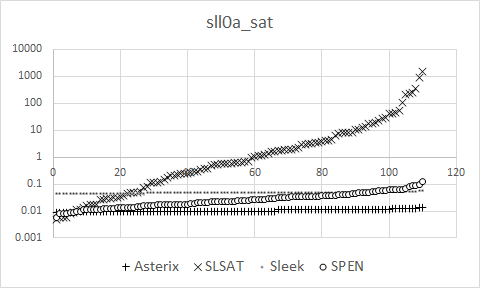
\includegraphics[width=0.46\textwidth]{sll0a_sat.png}
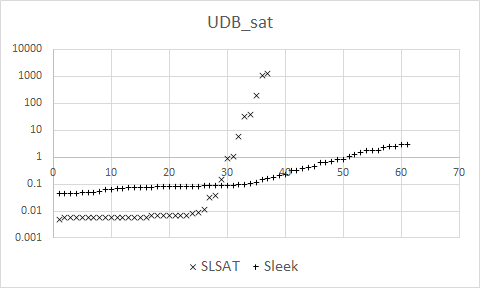
\includegraphics[width=0.46\textwidth]{UDB_sat.png}
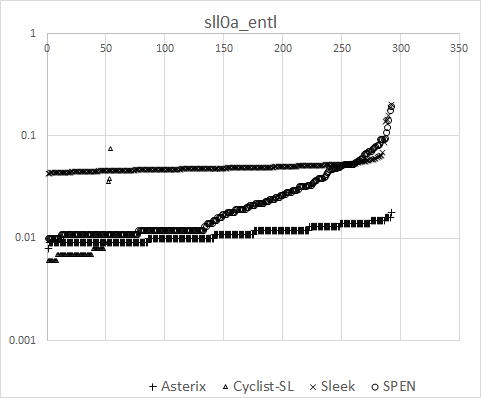
\includegraphics[width=0.46\textwidth]{sll0a_entl.png}
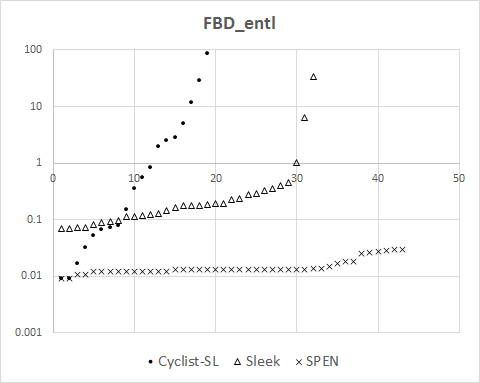
\includegraphics[width=0.47\textwidth]{FDB_entl.png}
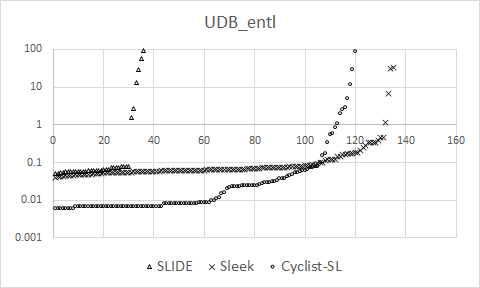
\includegraphics[width=0.6\textwidth]{UDB_entl.png}
\end{center}
\caption{Charts for the execution times in each division (vertical axis is log of time in sec.)}
\label{fig:charts}
\end{figure}


%%%%%%%%%%%%%%%%%%%%%%%%%%%%%%%%%%%%%%%%%%%%%%%%%%
\section{Conclusions and Perspectives}

\slcomp\ fulfilled its goals:
an interesting suite of SL problems is publicly available in a common format and
the maturity of solvers submitted for this competition has been proven.

\paragraph{Findings:}
The following additional goals were also reached:
\begin{itemize}
\item We achieved a first step in establishing a common format for the SL. 
This work revealed the features required by the existing solvers, e.g., the strong typing of formulas, the kind of inductive definitions handled, etc.
%% DONE: Reviewer 3: say which parts of the format need some readjustments (what are the expected evolutions ?).
Also, the use of the current format shows that it needs some readjustments to decrease its verbosity and to obtain a better integration in the semantics of the \smtlib\ format. 
The new features of the \smtlib 2 format, e.g., abstract data types and recursive function definitions, could facilitate the revision of the common format.

\item Some of the competing solvers have been improved (extensions, bugs fixed) during the preparation of this competition. They also gained experience with the preparation of a distribution for the \starexec\ platform. 
%
Note that the preparation of an version of a solver for \starexec\ was non-trivial. 
To avoid system-dependencies and to treat every participant in a competition equally, \starexec\ requires a 
statically-linked instance of a solver runnable in \starexec's Linux environment. Preparing such a version
of a solver was time-consuming and resulted in one intended participant's withdrawal. This problem
exists for first-time competitors in other \starexec-hosted competitions as well.

\item A community interested in such tools has been identified and informed about the status of the existing solvers.
This community could benefit from improving the tools built on the top of decision procedures for SL.

\item The \smtlib\ community discovered the status of the solvers for SL and became interested in this theory.

\item A interesting problem has been submitted to the \starexec\ platform by one solver, \textsc{SeLoger}~\cite{HasseIOP13}, initially submitted to \slcomp. 
%% DONE: Reviewer 3: rephrase 
This solver needs to have a batch execution in order to avoid the loading of the interpreter executing its binary (the solver needs a Windows platform) at each job.
This feature is different from the incremental mode provided by the \starexec\ platform. 
It requires to measure only the score obtained on a bunch of problems, without measuring the details on each problem. 

\end{itemize}


\paragraph{Future work:}
First of all, we are trying to reach a consensus for a good cadence of this competition. Yearly competitions could be very exciting for the first years, but may focus on engineering improvements rather than fundamental work. 
A good cadence may be, for example, alternating a competition year with a year of benchmark evaluation and improvement.
%% when solvers may be tested on the collected benchmarks and benchmarks may be fixed/annotated/studied.

In the intervening time to the next edition of the competition, several tasks are intended to be accomplished.
\begin{enumerate}
%\item The input format has to be standardized, based on the experience of the inaugural. 
%\fbox{Is there a need for change?}

\item The relationship of the SL theory to \smtlib\ must be understood. 
This may require alterations to the basic SL theory or designing an embedding of SL as an \smtlib\ theory.
The discussion group \url{sl2smtlib@googlegroups.com} has been opened for working out this relationship.
%% DONE: Added
The new features of the \smtlib 2 format, e.g., recursive function definitions, are very important for the SL theory.
The use of the \smtlib\ format for \slcomp\ is convenient because some SL solvers already deal with a combination of SL with theories currently available in \smtlib\, e.g., 
integer arithmetics theory~\cite{PerezR11}, array theory~\cite{BouajjaniDES12-vmcai}, set theory~\cite{PiskacWZ13}, etc.


\item With the experience of the current competition, the set of benchmarks has to be improved in the following directions:
\begin{itemize}
\item More benchmarks must be added in the existing divisions, especially the ones with smallest number of benchmarks. 
%% DONE: Reviewer 3: industrial benchmarks
Moreover, we have to increase the number of benchmarks coming from the software verification tools developed in academia or industry.
%% DONE: Reviewer 3: We added a comment on "Future work" paragraph about including more difficult problems (in size of the problem) in this division.
The easy divisions, i.e., \sllsat\ to \FDBent, should include more difficult problems to push at their limits the existing solvers.

\item Some new divisions will be introduced to take into account the needs of the software verification tools. For example, the combination of SL with integer arithmetics is used in tools that reason about the heap consumption.

\item The scoring system will be improved by assigning a difficulty to each benchmark problem. This should lead to a better evaluation of each solver.
%% DONE: Reviewer 3: How do you plan to assign a measure?
A classic way to assign a difficulty level is to take into account the size of the formulas and of the inductive definitions used in the problem. 
However, we think that for divisions like \UDBsat\ and \UDBent, an additional factor of difficulty is the number of fields of the data structure and the ``uniformity'' of its shape. 
For example, it seems to be easier to solve problems using \texttt{btree} definition than the \texttt{tll} definition.
\end{itemize}

\item The use of solvers in software verification tools requires improving solver capabilities such as
computing a witness for satisfiability problems,
providing unsatisfiability cores (i.e., diagnosis) or proofs,
and supporting abduction.

\item An interesting task is to find a way to measure individual solver improvement (in the face of a changing benchmark set), because this should encourage teams to work on both the engineering and the theoretical foundations of their tools.
% 

\item Finally, we should ease the task of entrants in this competition by providing, well in advance, clear rules, guidelines for solver preparation, pre-processors for their input language, etc. Many of these aspects were worked out in this first competition as participants were making their preparations.

\end{enumerate}

%\fbox{Announce the next competition?}

\section*{Acknowledgments}

The authors thank the contributors to this competition:
Nikos Gorogiannis, 
Juan Navarro Perez, 
Adam Rogalewicz, Ondrej Lengal, Tomas Vojnar, 
Wei Ngan Chin, Le Quang Loc, 
Radu Iosif, 
Andrey Rybalchenko, and
Constantin Enea.

We thank the  participants to the discussion list, especially 
Josh Berdine, John Brotherston, Christoph Hasse, and Thomas Wies, 
for their interesting comments on the input theory and format used in the competition.
We also thank reviewers of the paper for their interesting suggestions for improving its presentation.

%by institution
%%Nikos Gorogiannis, Middlesex University London
%%Juan Navarro Perez, University College London
%%Adam Rogalewicz, Ondrej Lengal, Tomas Vojnar, FIT, Brno University of Technology, IT4Innovations Centre of Excellence, Czech Republic
%%Wei Ngan Chin, Le Quang Loc,  National University of Singapore
%%Radu Iosif, VERIMAG, CNRS, France
%%Andrey Rybalchenko, Microsoft Research
%%Constantin Enea, Mihaela Sighireanu, University Paris Diderot and CNRS


%%%%%%%%%%%%%%%%%%%%%%%%%%%%%%%%%%%%%%%%%%%%%%%%%%
\bibliographystyle{plainbv}
\bibliography{bibliography}

\end{document}
